\documentclass[tikz,border=2pt,11pt]{standalone}
\usetikzlibrary{fit}
\usetikzlibrary{arrows.meta}
\usetikzlibrary{positioning}
\usetikzlibrary{shapes.geometric}
\usepackage{amsmath}
\usepackage{amssymb}
\usepackage{graphicx}
\usepackage{tikz}
\usepackage{xcolor}
\newcommand{\C}{\mathbb C}
\newcommand{\Z}{\mathbb Z}
\newcommand{\Q}{\mathbb Q}
\newcommand{\R}{\mathbb R}
\newcommand{\PP}{\mathbb P}
\newcommand{\A}{\mathbb A}
\newcommand{\cO}{\mathcal O}
\newcommand{\cH}{\mathcal H}
\newcommand{\cL}{\mathcal L}
\newcommand{\cF}{\mathcal F}
\newcommand{\cE}{\mathcal E}
\newcommand{\cD}{\mathcal D}
\newcommand{\sm}{\mathrm{sm}}
\DeclareMathOperator{\Spec}{Spec}
\DeclareMathOperator{\Proj}{Proj}
\DeclareMathOperator{\Sym}{Sym}
\DeclareMathOperator{\Pic}{Pic}
\DeclareMathOperator{\End}{End}
\DeclareMathOperator{\Hom}{Hom}
\DeclareMathOperator{\Hilb}{Hilb}
\DeclareMathOperator{\ch}{ch}
\DeclareMathOperator{\td}{td}
\DeclareMathOperator{\rk}{rk}
\DeclareMathOperator{\Gal}{Gal}
\DeclareMathOperator{\coker}{coker}
\DeclareMathOperator{\im}{im}
\begin{document}
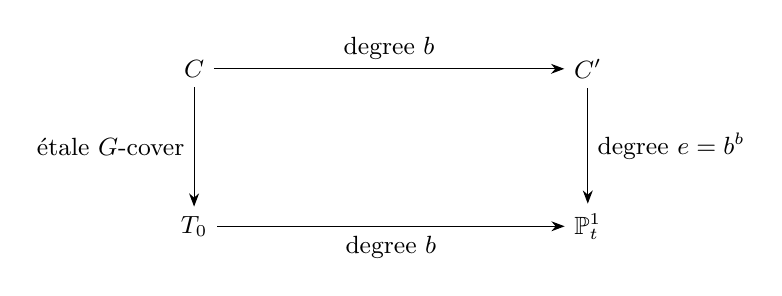
\begin{tikzpicture}[>=Stealth,every node/.style={font=\small}]
\node (C) at (0,2) {$C$};
\node (Cp) at (5,2) {$C'$};
\node (T) at (0,0) {$T_0$};
\node (P) at (5,0) {$\PP^1_t$};
\draw[->] (C)--node[above]{degree $b$}(Cp);
\draw[->] (C)--node[left]{\'etale $G$-cover}(T);
\draw[->] (Cp)--node[right]{degree $e=b^b$}(P);
\draw[->] (T)--node[below]{degree $b$}(P);
\end{tikzpicture}
\end{document}
